\documentclass[conference]{IEEEtran}
\renewcommand{\IEEEkeywordsname}{Keywords}

\usepackage{cite}
\usepackage{amsmath,amssymb,amsfonts}
\usepackage{algorithm2e}

\makeatletter
\newcommand{\removelatexerror}{\let\@latex@error\@gobble}
\makeatother
\newcommand{\casteljau}{%
\begingroup
\removelatexerror% Nullify \@latex@error
\begin{algorithm*}[H]
\caption{De Casteljau's Algorithm for Cubic Bézier Curves}\label{algo:de_casteljau}
\KwIn{Control points \(\mathbf{P}_0, \mathbf{P}_1, \mathbf{P}_2, \mathbf{P}_3 \in \mathbb{R}^2\) or \(\mathbb{R}^3\), parameter \(t \in [0, 1]\)}
\KwOut{Point \(\mathbf{B}(t)\) on the Bézier curve}

\BlankLine
\textbf{Step 1: Linear interpolation of the first level}  
\[
\mathbf{P}_{01} = (1-t) \mathbf{P}_0 + t \mathbf{P}_1
\]
\[
\mathbf{P}_{12} = (1-t) \mathbf{P}_1 + t \mathbf{P}_2
\]
\[
\mathbf{P}_{23} = (1-t) \mathbf{P}_2 + t \mathbf{P}_3
\]

\BlankLine
\textbf{Step 2: Linear interpolation of the second level}  
\[
\mathbf{P}_{012} = (1-t) \mathbf{P}_{01} + t \mathbf{P}_{12}
\]
\[
\mathbf{P}_{123} = (1-t) \mathbf{P}_{12} + t \mathbf{P}_{23}
\]

\BlankLine
\textbf{Step 3: Linear interpolation of the third level (final point)}  
\[
\mathbf{B}(t) = (1-t) \mathbf{P}_{012} + t \mathbf{P}_{123}
\]

\Return \(\mathbf{B}(t)\)
\end{algorithm*}
\endgroup}

% FOOTER
\makeatletter
%%%%%%%%% from https://tex.stackexchange.com/a/200330/161015
\def\ps@IEEEtitlepagestyle{% works only for the first page
    \def\@oddfoot{\customfootnote}%
    \def\@evenfoot{}%
}
\makeatother

\newcommand{\customfootnote}{Makalah IF2123 Aljabar Linier dan Geometri -- Teknik Informatika ITB -- Semester I Tahun 2024/2025\hfill}% define /edit here <<<<<<<<<<<<<<<

\usepackage{fancyhdr}
\fancyhf{}
\renewcommand{\headrulewidth}{0pt}
\fancypagestyle{GlobalFootnote}{%
    \lfoot{\customfootnote} 
}
\pagestyle{GlobalFootnote} % style for following pages

\usepackage{graphicx}

\usepackage{textcomp}

\usepackage{hyperref}
\usepackage{xcolor}

\def\BibTeX{{\rm B\kern-.05em{\sc i\kern-.025em b}\kern-.08em
    T\kern-.1667em\lower.7ex\hbox{E}\kern-.125emX}}
\begin{document}

\title{Implementation of Vector, Linear Transformation, and Quaternion Algebra in the Creation and Manipulation of Bézier Curves for 3D Computer Graphics}

\author{{Z. Nayaka Athadiansyah -- 13523094\textsuperscript{1,2}} \\
\IEEEauthorblockA{\textit{Program Studi Teknik Informatika} \\
\textit{Sekolah Teknik Elektro dan Informatika}\\
\textit{Institut Teknologi Bandung, Jl. Ganesha 10 Bandung 40132, Indonesia} \\
\textit{\color{blue} \textsuperscript{1}\href{mailto:13523094@std.stei.itb.ac.id}{13523094@std.stei.itb.ac.id}}, \textit{\color{blue} \textsuperscript{2}\href{mailto:nayaka.zna@gmail.com}{nayaka.zna@gmail.com}}
}
}

\maketitle

\begin{abstract}
    This paper aims to provide a simple demonstration for Bézier curve and linear transformations in 3D computer graphics. Vectors are implemented to generate 3D Bézier curves, while linear transformation such as reflection, scaling, and rotation are implemented using transformation matrices and quaternions to manipulate the curves. Since Bézier curves are affine combinations of its control points, which can be represented as vectors, we can apply linear transformations to its control points in order to apply those transformations to the whole curve. A demonstration is carried by a simple OpenGL-based GUI program made using GLFW and ImGUI in Python.
\end{abstract}

\begin{IEEEkeywords}
3D computer graphics, bézier curve, linear transformation, quaternion algebra, vector mathematics
\end{IEEEkeywords}

\section{Introduction}Computer graphics has been a broad and rapidly advancing field of research since the 1960s, contributing significantly to innovations across various fields of study\cite{hughes}, such as computer-aided design, virtual reality, and video game development. Computer graphics refers to the science and methods of creating and manipulating visual representations of computer objects\cite{eck}. It also includes the study of visual human-computer interaction, which involves the use of peripheral devices such as visual display units (VDUs) and keyboards to facilitate interaction. It is a multidisciplinary field of research involving engineering, physics, mathematics, computer science, visual art, and behavioral science \cite{hughes}. In this paper, we will limit our discussions to 3D computer graphics exclusively. Hence, whenever we mention "computer graphics," we refer to "3D computer graphics".

\begin{figure}[htb!]
    \centering
    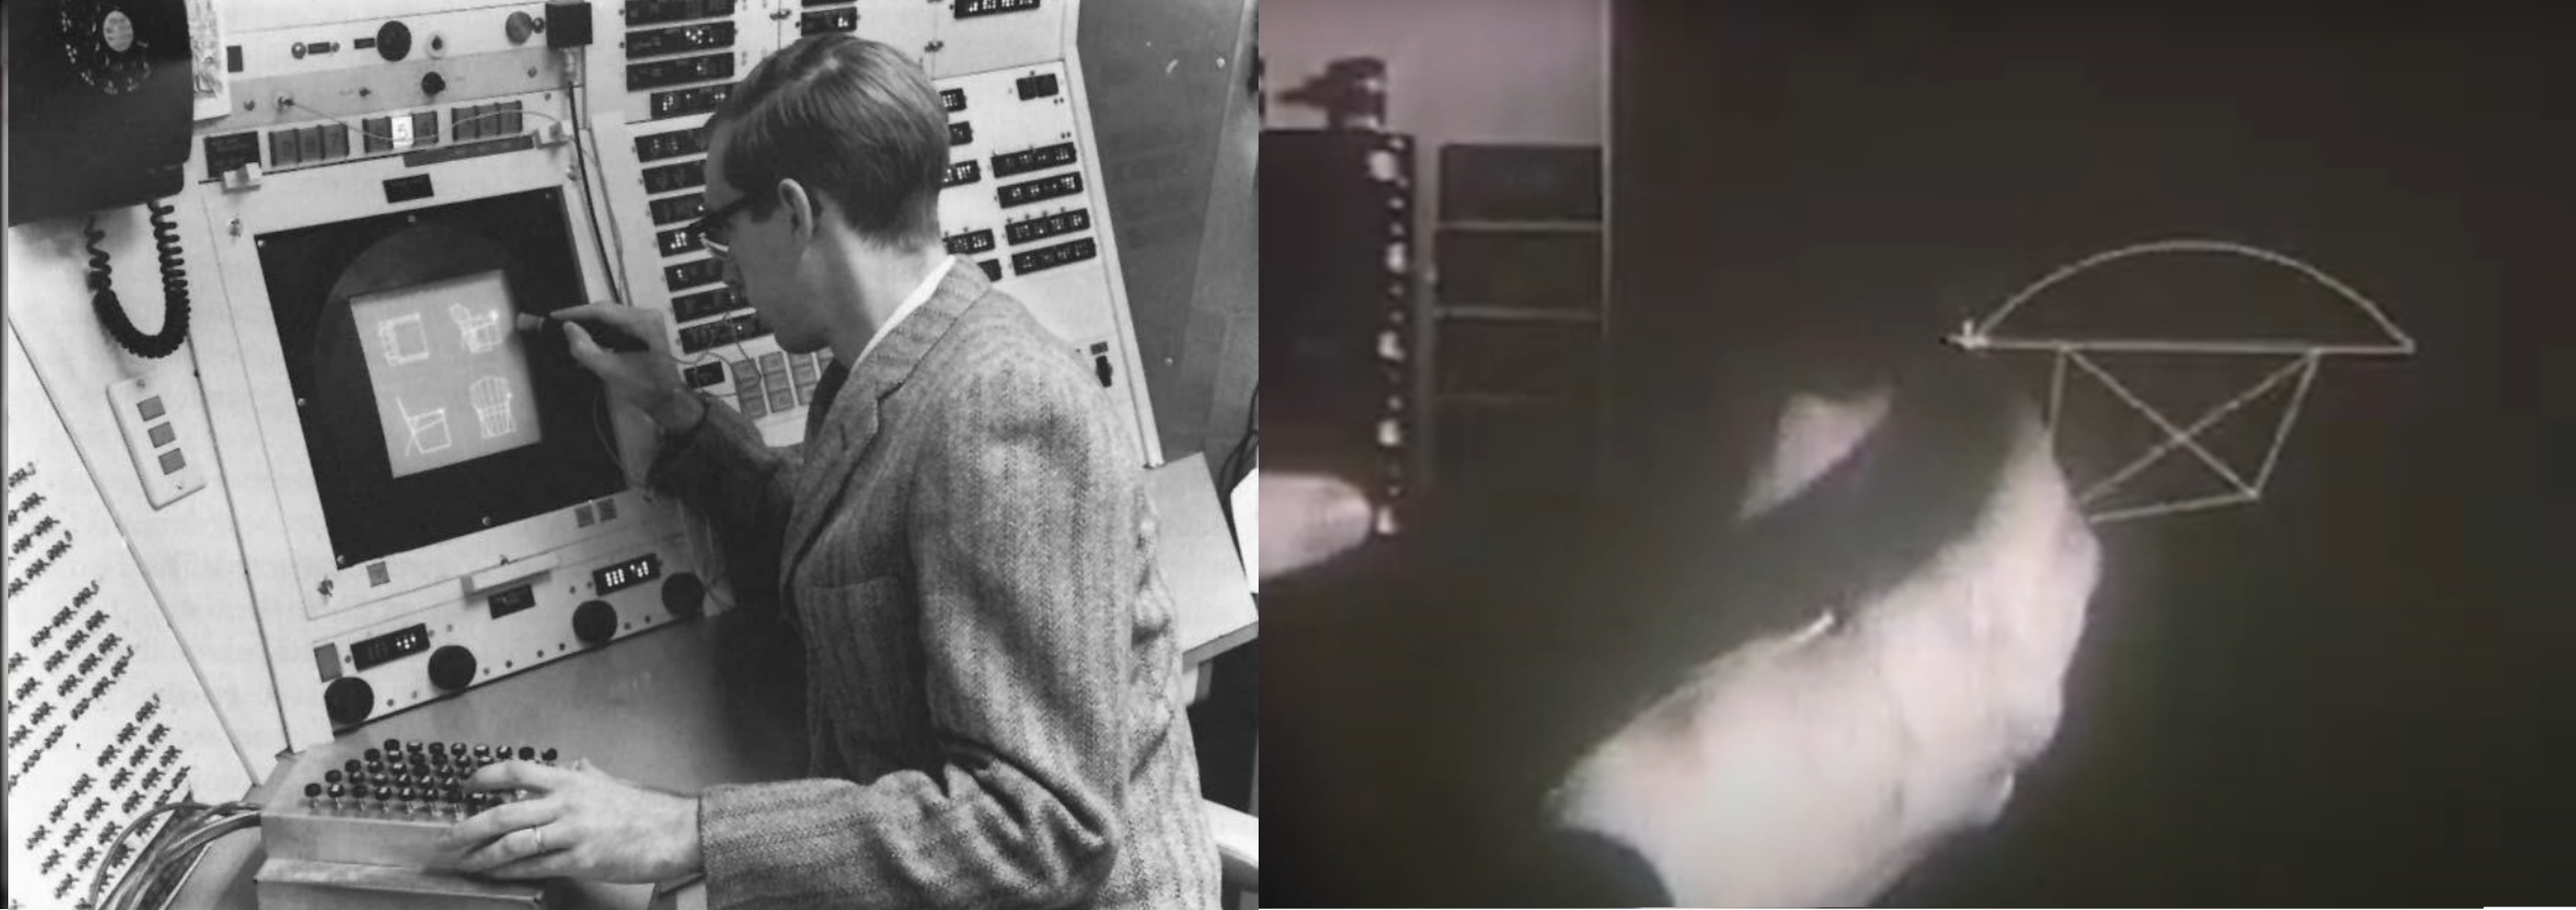
\includegraphics[width=1\linewidth]{sketchpad1.png}
    \caption{A 1963 demonstration of Ivan Sutherland's \textit{Sketchpad}. Source: MIT Lincoln Laboratory}
\end{figure}
In 1963, Ivan Sutherland, an electrical engineering Ph.D. student at MIT Lincoln Laboratory, invented the \textit{Sketchpad}. This innovative computer program marked the beginning of developments in computer graphics\cite{hci}\cite{acm}. \textit{Sketchpad} significantly demonstrated the initial application of a graphical user interface (GUI) and was an early form of computer-aided design (CAD) program, as it was specifically designed to create and interactively modify graphical objects represented as geometrical shapes. The program, written for an MIT Lincoln Laboratory TX-2 computer, involved the usage of a light pen as an input device enabling the creation of geometrical figures using line drawings instead of prompting through keyboard input \cite{sutherland}, making it a real-time interactive GUI program.

\begin{figure}[htb!]
    \centering
    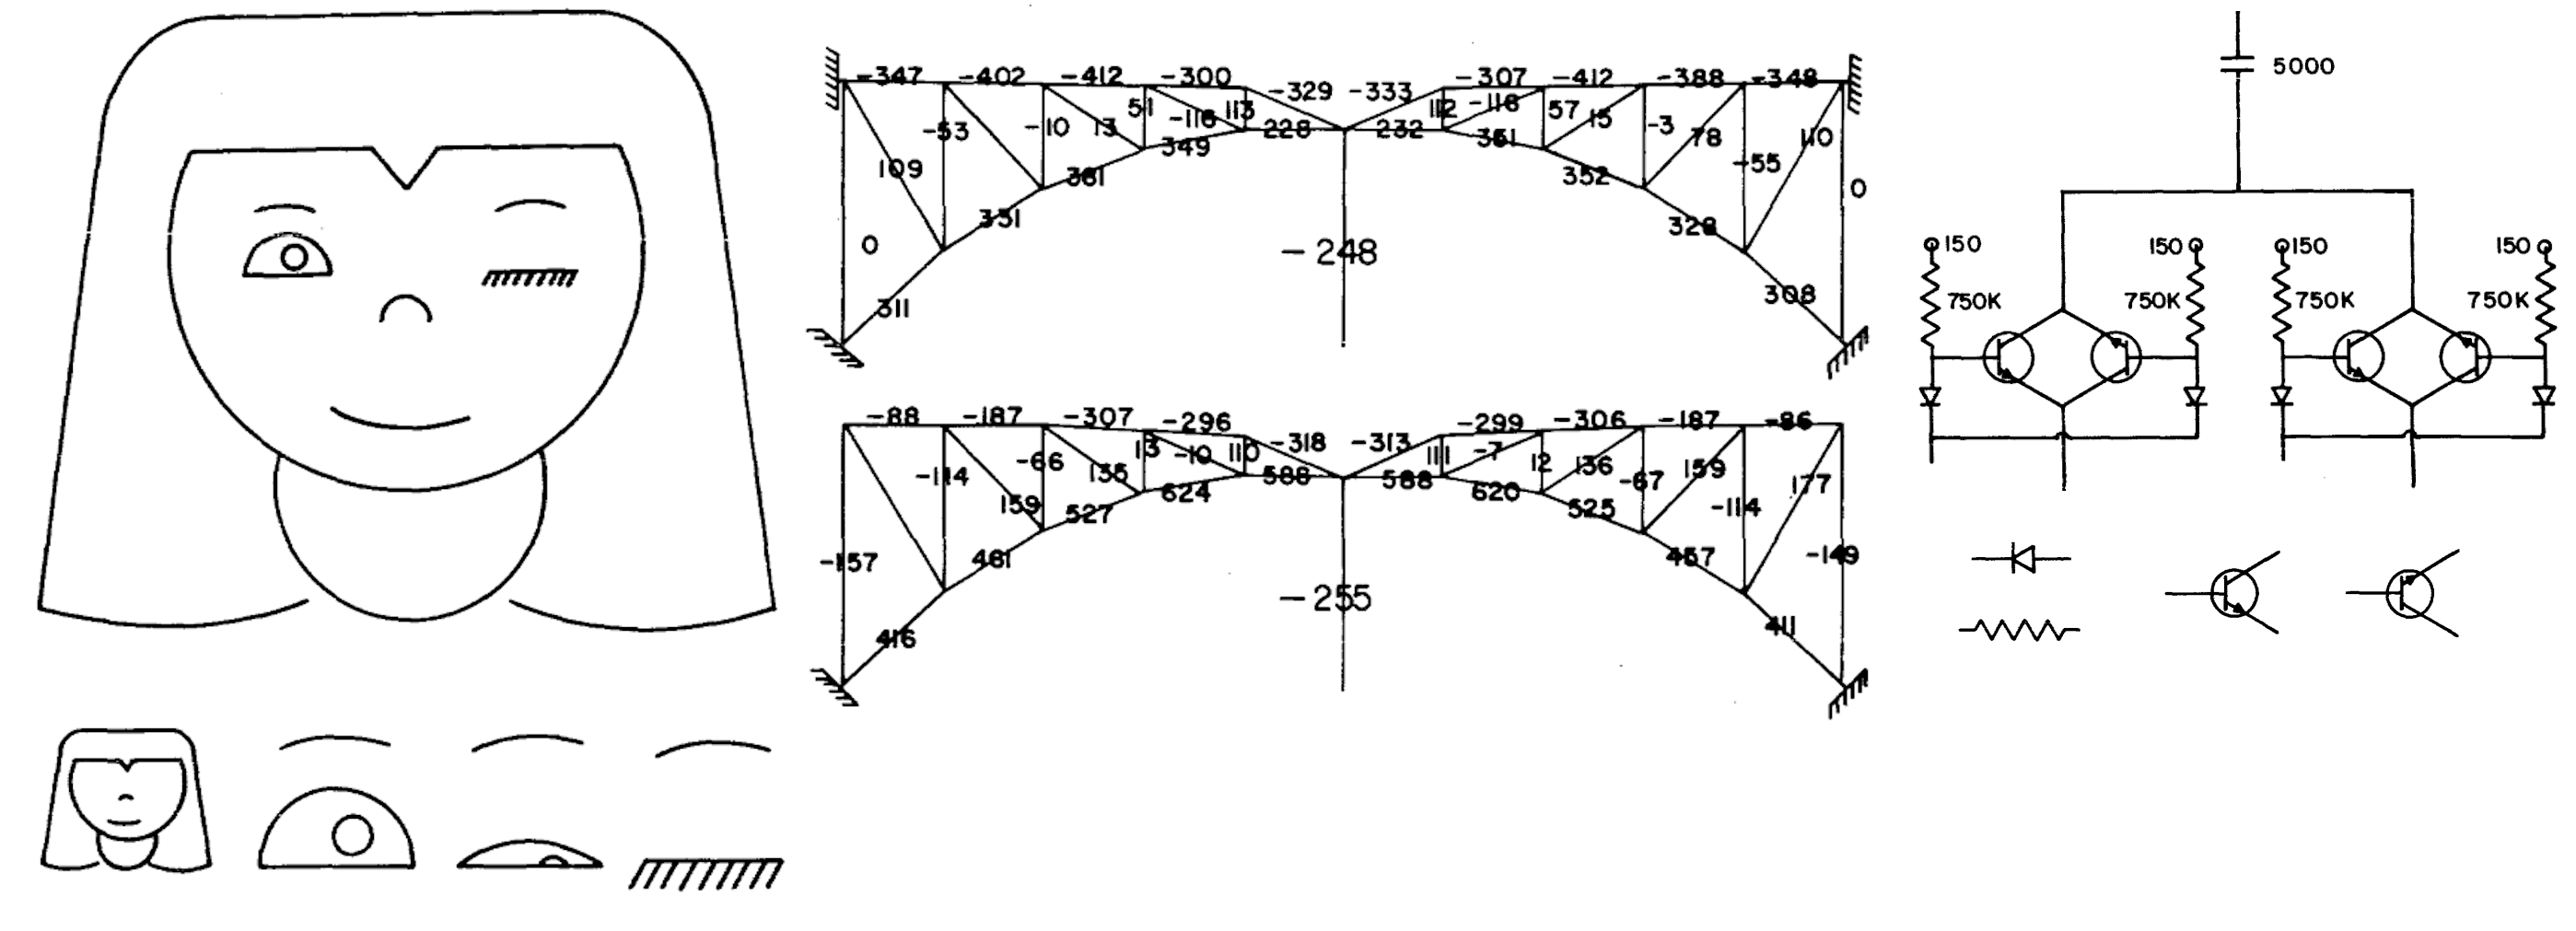
\includegraphics[width=1\linewidth]{sketchpad2.png}
    \caption{Several examples of graphical illustrations created in \textit{Sketchpad} (from left): the winking lady 
    "Nefertite" and her graphical component parts; truss diagrams of a cantilever and an arch bridge, with calculations 
    of internal forces in the members; and an electrical circuit. Source: \cite{sutherland}}
\end{figure}
\textit{Sketchpad} users could reuse and combine existing graphical objects to form a new one, letting the users structure its graphical objects hierarchically. Users could also create shapes using constraints. For instance, users could create a parallelogram by constraining the pair of sides to be parallel and having equal length. Sutherland's invention revolutionized human-computer interaction, object-oriented programming, and, especially, computer graphics modeling. Later on, Sutherland and David Evans, a computer science professor from the University of Utah, established Evans and Sutherland to manufacture hardware capable of running computer graphics programs. Due to his innovations, he was awarded the Turing Award in 1988\cite{acm}.


The next decades saw plentiful breakthroughs in the field. Better imagery could be generated due to the development of new methods and algorithms, including Z-buffer algorithm, anti-aliasing, Phong shading, and ray tracing\cite{history}. With a growing enthusiasm for research in computer graphics the Special Interest Group on Computer Graphics and Interactive Techniques (SIGGRAPH) was founded in 1974 as a platform for experts in computer graphics\cite{siggraph}. In the 1980s and 1990s, milestones in computer graphics included the release of 3D computer-animated films such as "Tron," "Toy Story," and "Jurassic Park"; the introduction of 3D modeling software such as Autodesk 3Ds Max and Maya and frameworks such as OpenGL and Direct3D; and the emergence of graphical processing units (GPUs) from companies like NVIDIA\cite{history}\cite{cgi-movie}. These advancements laid the foundations for cutting-edge technologies in the field used today that can be seen everywhere, from entertainment, engineering, medical science, and many electronic appliances that we use daily.

One of the prominent concepts widely used in computer graphics is the Bézier curve. It was discovered in 1962 by the French engineer Pierre Bézier---hence its name. The mathematical groundwork to create such curve, de Casteljau's algorithm, had been discovered earlier in 1959 by Paul de Casteljau, a French mathematician \cite{bezier}. These curves are defined by a parametric equation and a set of control points, with two points acting as the both ends of the curve while the rest acts as "weights". Bézier curves can also be extruded or converted into meshes to create solid object models. Bézier curves are commonly available in computer graphics software, especially in 3D-modeling software like Blender and vector graphics software such as Adobe Illustrator. 

In this paper, we will discuss about creating Bézier curves in $\mathbb{R}^3$ by modeling its control point as vectors and manipulating it with linear transformations and quaternions. 

\section{Theoretical Foundation}
\subsection{Vector} 
Vectors are the elements of a vector space \cite{strang}. In the context of computer graphics, we talk about Euclidean vectors in $\mathbb{R}^3$, which can be represented graphically as an arrow pointing to its direction with a length corresponding to its magnitude. A vector $v$ can be denoted as an ordered tuple of three numbers, a column matrix, or it can also be written using unit notation, in which we make use of the standard basis of $\mathbb{R}^3$: $\hat{i} = (1, 0, 0)$, $\hat{j} = (0, 1, 0)$, and $\hat{k} = (0, 0, 1)$,
\begin{equation}
    \mathbf{v} = (v_x, v_y, v_z) = \begin{bmatrix}v_x \\ v_y \\ v_z \end{bmatrix} = v_x \hat{i} + v_y \hat{j} + v_z \hat{k},
\end{equation}
where $v_x$, $v_y$, and $v_z$ are its components along $x$, $y$, and $z$ axes, respectively \cite{lengyel}. A vector's magnitude (denoted as $|\mathbf{v}|$) can be calculated using the Pythagorean theorem as
\begin{equation}
    |\mathbf{v}| = \sqrt{v_x^2 + v_y^2 + v_z^2}. 
\end{equation}

A vector's magnitude can be scaled by multiplying the vector by a scalar $k \in \mathbb{R}$. Mathematically,
\begin{equation}
    k\mathbf{v} = k \begin{bmatrix}v_x \\ v_y \\ v_z \end{bmatrix} = \begin{bmatrix} kv_x \\ kv_y \\ kv_z \end{bmatrix}. 
\end{equation}

Graphically, multiplying a vector by a negative scalar results in inverting its direction. Scalar multiplication is distributive towards scalar and vector addition, 
\begin{align}
    (k + \ell)\mathbf{v} = k\mathbf{v} + \ell\mathbf{v} \\
    k(\mathbf{u} + \mathbf{v}) = k\mathbf{u} + k\mathbf{v}
\end{align}
 and associative,
\begin{equation}
    (k\ell)\mathbf{v} = k (\ell\mathbf{v}).
\end{equation}
Using scalar multiplication and a vector's magnitude, we can normalise it i.e. turning the vector's magnitude into $1$ by using the formula
\begin{equation}
    \hat{v} = \frac{1}{|\mathbf{v}|} \mathbf{v}.
\end{equation}
Since the magnitude of vector $\mathbf{v}$ is $|\mathbf{v}|$, this formula essentially transforms the vector's magnitude into $|\mathbf{v}| \cdot \dfrac{1}{|\mathbf{v}|} = 1$ while preserving its orientation \cite{lengyel}. The vector $\hat{v}$ is called the unit vector in the direction of $\mathbf{v}$.

Addition between two (or more) vectors can be performed by adding the corresponding components, i.e.
\begin{equation}
    \left( \mathbf{u} = \begin{bmatrix} u_x \\ u_y \\ u_z \end{bmatrix} \ \land \ \mathbf{v} = \begin{bmatrix} v_x \\ v_y \\ v_z \end{bmatrix} \right) \implies \mathbf{u} + \mathbf{v} = \begin{bmatrix} u_x + v_x \\ u_y + v_y \\ u_z + v_z \end{bmatrix}. 
\end{equation}
Vector addition is commutative,
\begin{equation}
    \mathbf{u} + \mathbf{v} = \mathbf{v} + \mathbf{u},
\end{equation}
and associative,
\begin{equation}
    \mathbf{u} + (\mathbf{v} + \mathbf{w}) = (\mathbf{u} + \mathbf{v}) + \mathbf{w}.
\end{equation}
In its graphical representation, vector addition can be done by placing the tail of the second vector to the first vector's head.

% TODO: add illustrations using TiKz

\subsection{Linear Transformation} 
The linear transformation from $\mathbb{R}^n$ to $\mathbb{R}^m$ is defined as the function $T$ that transform every vector $\mathbf{v}$ in $\mathbb{R}^n$ to a corresponding vector, $T(\mathbf{v})$ in $\mathbb{R}^m$ \cite{strang}. A \textbf{linear} transformation shall satisfy the condition
\begin{equation}
    T(\mathbf{v} + \mathbf{w}) = T(\mathbf{v}) + T(\mathbf{w}) \qquad \text{and} \qquad T(c\mathbf{v}) = cT(\mathbf{v}) 
\end{equation}
for all $\mathbf{v}, \mathbf{w} \in \mathbf(V)$, and $k \in \mathbb{R}$ \cite{strang}. Note that if the basis vectors of $\mathbf{V}$ is $v_1, v_2, \ldots, v_n$, then every vector $\mathbf{v} \in \mathbf{V}$ can be expressed as a linear combination of them,
\begin{equation}
    \mathbf{v} = c_1 v_1 + c_2 v_2 + \ldots c_n v_n.
\end{equation}
When we want to apply a linear transformation to a particular vector of a vector space $\mathbf{V}$, it is more helpful to consider the general case: \textit{how does the linear transformation apply to the basis vectors of} $\mathbf{V}$? 

Since every vector in $\mathbf{V}$ can be expressed in terms of its basis vectors, knowing the images of new basis vectors under the linear transformation is sufficient to determine the transformed vector. Suppose
\begin{align*}
    T(\mathbf{v}_1) &= a_{11} \mathbf{v}_1 + a_{21} \mathbf{v}_2 + \cdots + a_{n1} \mathbf{v}_n \\
    T(\mathbf{v}_2) &= a_{12} \mathbf{v}_1 + a_{22} \mathbf{v}_2 + \cdots + a_{n2} \mathbf{v}_n \\
    \vdots \\
    T(\mathbf{v}_n) &= a_{1n} \mathbf{v}_1 + a_{2n} \mathbf{v}_2 + \cdots + a_{nn} \mathbf{v}_n.
\end{align*}

We can rewrite this system of equations into
\begin{equation}
    \begin{bmatrix} T(\mathbf{v}_1) \\ T(\mathbf{v}_2) \\ \vdots \\ T(\mathbf{v}_n)\end{bmatrix} = 
\underbrace{\begin{bmatrix}
    a_{11} & a_{21} & \cdots & a_{n1} \\
    a_{12} & a_{22} & \cdots & a_{n2} \\
    \vdots & \vdots & \ddots & \vdots \\
    a_{1n} & a_{2n} & \cdots & a_{nn}
\end{bmatrix}}_{A}
\begin{bmatrix} \mathbf{v}_1 \\ \mathbf{v}_2 \\ \vdots \\ \mathbf{v}_n \end{bmatrix}
\end{equation}

The matrix $A$ is called the \textit{transformation matrix} of $T$. In other words, $T(\mathbf{v})$ can be acquired from multiplying $A$ and $\mathbf{v}$ \cite{lengyel}.

There are several common linear transformation matrices \cite{lengyel}. The reflection matrices
\[ R_{xy} = 
\begin{bmatrix}
    1 & 0 & 0 \\
    0 & 1 & 0 \\
    0 & 0 & -1 
\end{bmatrix},
\quad
R_{xz} = 
\begin{bmatrix}
    1 & 0  & 0 \\
    0 & -1 & 0 \\
    0 & 0  & 1 
\end{bmatrix},
\]
\[
\text{and }
R_{yz} = 
\begin{bmatrix}
   -1 & 0 & 0 \\
    0 & 1 & 0 \\
    0 & 0 & 1 
\end{bmatrix}
\]

reflects a vector across the $xy$, $xz$, and $yz$-plane, respectively. Scaling a vector $\mathbf{v}$ by a scalar $k$ can be acquired by multiplying them, but we can also view it as a matrix multiplication,
\[
k\mathbf{v}
= \begin{bmatrix} k\mathbf{v_x} \\ k\mathbf{v_y} \\ k\mathbf{v_z} \end{bmatrix}
=
\begin{bmatrix}
    k & 0 & 0 \\
    0 & k & 0 \\
    0 & 0 & k
\end{bmatrix}
\begin{bmatrix} \mathbf{v_x} \\ \mathbf{v_y} \\ \mathbf{v_z} \end{bmatrix}.
\]


When the diagonal entries are not equal, we get a nonuniform scale matrix,
\[
\begin{bmatrix}
    k_x & 0 & 0 \\
    0 & k_y & 0 \\
    0 & 0 & k_z
\end{bmatrix}.
\]

Next, the matrix for shear mapping, in which points lying on an axis stays the same while the rest is shifted parallel towards the axis is given by
\[
\begin{bmatrix}
     1 & xy & xz \\
    yx &  1 & yz \\
    zx & zy & 1
\end{bmatrix}
\]

Lastly, the transformation matrix to rotate a vector in the angle of $\theta$ about an axis defined by a unit vector $(x, y, z)$ is
\[
{\begin{bmatrix}
x^2(1-c_\theta )+c_\theta &yx(1-c_\theta )-zs_\theta &zx(1-c_\theta )+ys_\theta \\
xy(1-c_\theta )+zs_\theta &y^2(1-c_\theta )+c_\theta &zy(1-c_\theta )-xs_\theta \\
xz(1-c_\theta )-ys_\theta &yz(1-c_\theta )+xs_\theta &z^2(1-c_\theta )+c_\theta 
\end{bmatrix}}
\]
where $c_\theta = \cos \theta$ and $s_\theta = \sin \theta$ \cite{lengyel}. 

\subsection{Affine Transformation and Combination}

The affine transformation from $\mathbb{R}^n$ to $\mathbb{R}^m$ is defined as the function $T$ in the form of
\begin{equation}
    T(x) = A\mathbf{x} + \mathbf{b},
\end{equation}
where $A$ is a linear transformation (which, as we have shown, can be represented by its transformation matrix) and $\mathbf{b} \in \mathbb{R}^m$, which can be seen as the translation vector. Linear transformations are part of \textit{affine} transformations, which preserves lines and parallelism \cite{affine1}. It can be seen that the linear transformation is the special case when $\mathbf{b} = \mathbf{0}$.

Let $t_0, \ldots, t_k \in \mathbb{R}$ such that $\sum_{i=0}^k t_i = 1$. Given the vectors $x_0$, \ldots , $x_k \in \mathbb{R}^n$, then $\sum_{i=0}^k t_i\mathbf{x}_i$ is an affine combination of them\cite{affine2}. It can be proven that when an affine transformation is applied to an affine combination, the image can be calculated by applying the same affine transformation to the individual vectors, since
\begin{align}
    T\left(\sum_{i=0}^k t_i\mathbf{x}_i\right) &= A{\sum_{i=0}^k t_i \mathbf{x}_i} + \mathbf{b} \notag \\
    &= A\sum_{i=0}^k t_i\mathbf{x}_i + \sum_{i=0}^k t_i \mathbf{b} \notag \\
    &= \sum_{i=0}^k t_i A\mathbf{x}_i + \sum_{i=0}^k t_i \mathbf{b} \notag \\
    &= \sum_{i=0}^k t_i (A\mathbf{x}_i + \mathbf{b}) \notag \\
    &= \sum_{i=0}^k t_i T\left(\mathbf{x}_i\right)
\end{align}

\subsection{Quaternion} 
Quaternions, usually denoted as $q$, are elements of a 4-dimensional vector space, $\mathbb{H}$, over $\mathbb{R}$ \cite{lengyel}\cite{quat}. A quaternion can be expressed in the form 
\begin{equation}
    q = \langle w, x, y, z \rangle = w + xi + yj + zk, 
\end{equation}
where $w, x, y,$ and $z$ are real numbers, while the imaginary components $i, j$, and $k$ is defined by the relationship
\begin{equation}
    i^2 = j^2 = k^2 = ijk = -1.
\end{equation}

The imaginary components are also related to each other as
\begin{align} 
    ij &= -ji = k, \label{eq:q1}\\
    jk &= -kj = i, \label{eq:q2}\\
    ki &= -ik = j. \label{eq:q3}
\end{align}

We can also view $w$ as a scalar and $xi + yj + zk$ as a vector in $\mathbb{R}^3$. When $w = 0$, it becomes a regular 3-dimensional vector. Quaternions of this particular kind are \textit{pure} quaternions. 

One of the main properties of quaternions are \textit{norms}, the 4-dimensional counterpart of the magnitude of 3-dimensional vectors, which is a real number defined as
\begin{equation}
    |q| = \sqrt{w^2 + x^2 + y^2 + z^2}.
\end{equation}

Let $q_1 = w_1 + x_1j + y_1j + z_1k$ and $q_2 = w_2 + x_2j + y_2j + z_2k$. Addition and subtraction between two quaternions $q_1$ and $q_2$ is defined as
\begin{equation}
    \small
    {q_1} \pm {q_2} = (w_1 + w_2) + (x_1 + x_2)i + (y_1 + y_2)j + (z_1 + z_2)k.
\end{equation}

Addition and subtraction between quaternions are commutative and associative. We now introduce ourselves to quaternion multiplication, which are defined as
\begin{align}
    q_1 q_2 &= (w_1 + x_1j + y_1j + z_1k)(w_2 + x_2j + y_2j + z_2k) \notag \\
    &= (w_1w_2 - x_1x_2 - y_1y_2 - z_1z_2) \notag \\
    & + (w_1x_2 + x_1w_2 + y_1z_2 - z_1y_2)i \notag \\
    & + (w_1y_2 - x_1z_2 + y_1w_2 + z_1x_2)j \notag \\
    & + (w_1z_2 + x_1y_2 + y_1x_2 + z_1w_2)k.
\end{align}
which can be viewed as if we were distributing each component of $q_1$ to $q_2$, akin to applying the distributive law for multiplication in arithmetics, while considerating the identities in equation \ref{eq:q1}, \ref{eq:q2}, and \ref{eq:q3}.

The \textit{conjugate} of a quaternion $q = w + xi + yj + zk$, denoted as $q^*$ or $\bar{q}$, is defined by
\begin{equation}
    q^* = \overline{q} = w - xi - yj - zk
\end{equation}

One of the interesting results from this is that
\begin{align}
    q \cdot q^* &= (w + xi + yj + zk)(w - xi - yj - zk) \notag \\
    &= (w^2 + x^2 + y^2 + z^2) \notag \\
    &= + (-wx + wx - yz + zy)i \notag \\
    &= + (-wy + xz - yw - zx)j \notag \\
    &= + (-zw - xy - yx + zw)k \notag \\
    &= w^2 + x^2 + y^2 + z^2 \notag \\
    &= |q|^2
\end{align}

This result can be used to derive for the formula of the \textit{multiplicative inverse} of a nonzero quaternion, $q^{-1}$. Since $q \cdot q^{-1} = 1$ by definition, we get
\begin{equation}
    q^{-1} = \frac{q^*}{|q|^2}
\end{equation}
because $qq^* = |q|^2/|q|^2 = 1$.

Quaternions with norm of $1$ are unit quaternions, which can be represented as
\begin{equation}
    q = \cos \theta + \hat{\mathbf{u}} \sin \theta,
\end{equation}
where $\hat{\mathbf{u}}$ is a 3-dimensional normal vector. Similarly,
\begin{equation}
    q^{-1} = \cos \theta - \hat{\mathbf{u}} \sin \theta.
\end{equation}
Using this form, we can rotate any vector $\mathbf{v}$ with a given angle. Let $\mathbf{u}$ be a vector in the line of the axis of rotation of our choice such that the normal vector in its direction is $\hat{\mathbf{u}}$ and let $2\theta$ be the counterclockwise rotation angle. Now, we can express the vector $\mathbf{v}$ as a pure quaternion by writing it as $p = 0 + \mathbf{v}$. The rotated vector $\mathbf{v'}$ in the form of pure quaternion $p' = 0 + \mathbf{v'}$ can be acquired through the equation
\begin{equation}
    p' = qpq^{-1}
\end{equation}

\subsection{Comparation of 3-Dimensional Rotation Formalisms}
There are three common 3-dimensional rotation formalisms which can be converted into one another, namely rotation matrices, Euler angles, and quaternions. \cite{rot} provides a thorough analysis on comparing their performances. The three of them equally have a time complexity of $O(n)$. The rotation matrix has the biggest memory usage, since they need to store the $9$ elements of the $3 \times 3$ matrix, while Euler angles only need to store $3$ values, whereas quaternions require to store $4$ values. Additionally, composing a unit quaternion takes lesser operations compared to rotation matrix and Euler angles.

Euler angles, unfortunately, suffer from a phenomenon commonly known as the gimbal lock, in which. Moreover, the extensive calculation in rotation matrices might cause errors due to truncation or rounding. Thus, in this paper we will use quaternions for rotating Bézier curves.

\subsection{Bézier Curve} 
Bezier curves are parametric curves defined by a set of control points and a parametric equation. These particular kind of curves are widely used in computer graphics because it enables the creation of smooth curves for modeling. The first and last control points acts as the curve initial and final point, while the rest acts as weights that shapes the curve's curvature.

A Bézier curve has a degree, a quantity related to the amount of its control points. Given a set of $n+1$ control points, a Bézier curve of degree $n$ is defined by the parametric equation
\begin{equation}
    \mathbf{B}(t) = \sum_{i=0}^n b_{i,n}(t) \mathbf{P}_i, \quad t \in [0, 1],
\end{equation}
where $b_{i, n}$ is the Bernstein basis polynomial\cite{galier}
\begin{equation}
    b_{i,n}(t) = \binom{n}{i} t^i (1-t)^{n-i}
\end{equation}
and 
\begin{equation}
    \binom{n}{i} = \frac{n!}{i!(n-i)!}
\end{equation}
is the binomial coefficient. We will limit the scope of Bézier curve in this paper to cubic Bézier curves as they are the most commonly used type of Bézier curves in computer graphics. The method to create the Bézier curve graph is called de Casteljau's algorithm \cite{galier}. It recursively performs linear interpolation between the control points to generate a smooth graph of a Bézier curve.

\begin{figure}[htb!]
    \centering
    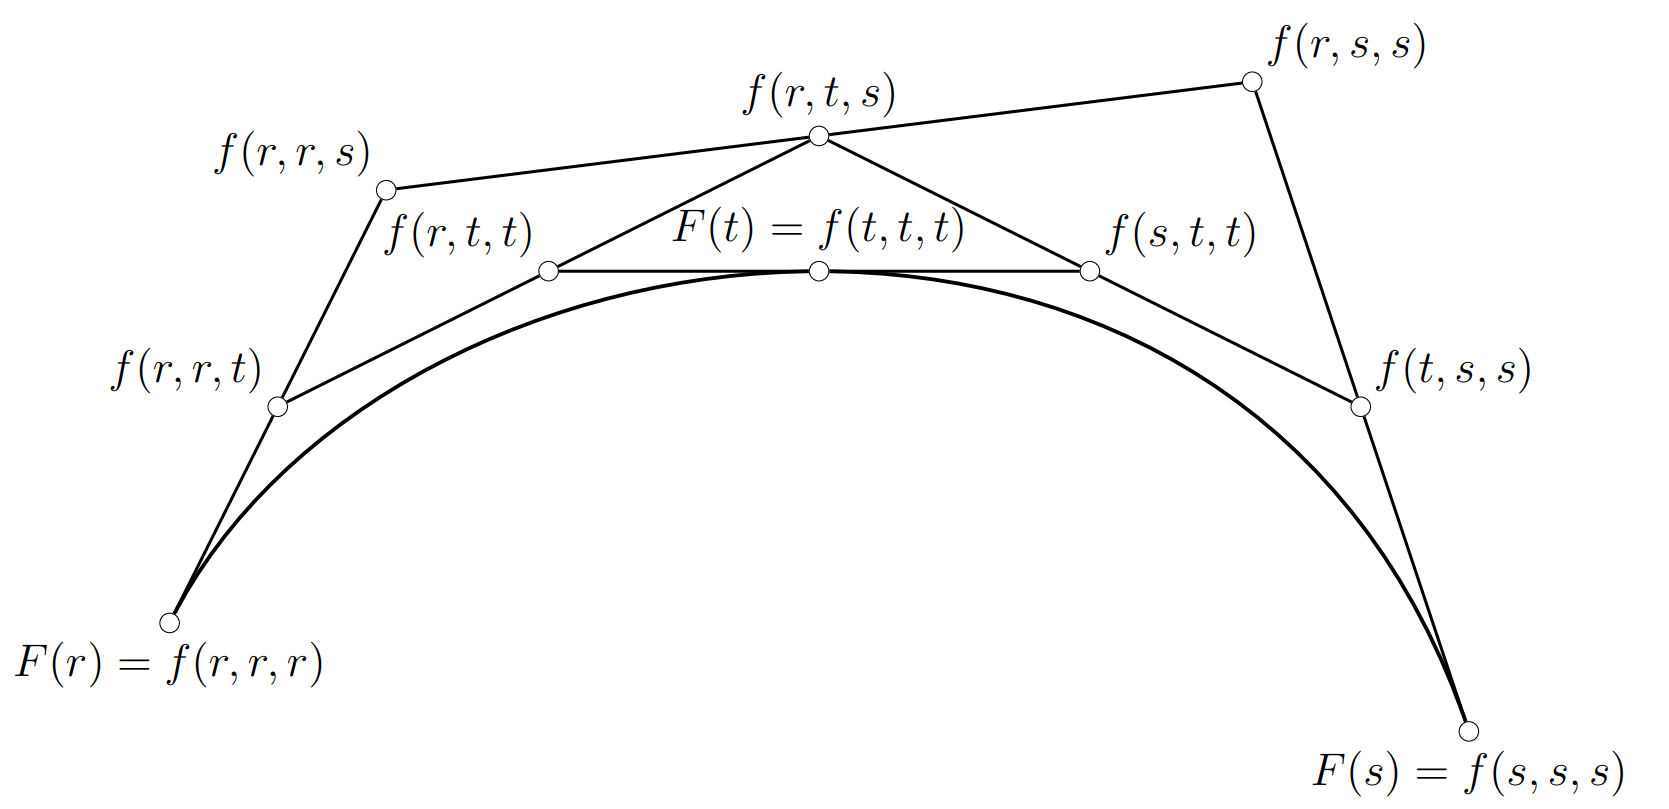
\includegraphics[width=0.75\linewidth]{casteljau.png}
    \caption{An illustration of de Casteljau's algorithm. Source: \cite{galier}}
\end{figure}

\newpage
The algorithm can be implemented as follows:
\casteljau

The variable $t$ can be seen as "time", where $t = 0$ at $\mathbf{P}_0$ and $t = 1$ at $\mathbf{P}_n$. 

\section{Analysis}
To demonstrate Bézier curve generation and manipulation, we will create a program in Python using OpenGL, assisted with the libraries GLFW and ImGUI. NDArray and trigonometric functions from NumPy is also used. For demonstration purpose, we will use cubic Bézier curve. The four control points can be seen as vectors. We then apply de Casteljau's algorithm to generate the Bézier curve into the display.

It can be shown that Bézier curves are affine combinations. This is done by showing that the Bernstein basis polynomial satisfy the condition for an affine combination. From the binomial expansion formula, we have
\begin{equation}
    (x + y)^n =  \sum_{i=0}^n \binom{n}{i} x^i y^{n-i}.
\end{equation}
Hence, the sum of Bernstein basis polynomial from degree $0$ to the $n$-th degree is
\begin{equation}
    \sum_{i=0}^n b_{i,n}(t) = \sum_{i=0}^n \binom{n}{i} t^i (1-t)^{n-i} = (t + 1 - t)^n = 1
\end{equation}
% proof

Hence, we can apply linear transformations to each of the control points to apply the transformation to the whole Bézier curve. Additionally, we will use quaternions to perform rotation.

The program interface comprises two main parts: the main window and the control panel. The main window acts as the Bézier curve’s display, giving dynamical 3D visualization space, and observing the possibility of real-time transformations in it. From this window, it becomes achievable to view the geometry of the curve from a clear and unambiguous perspective, therefore facilitating an easy analysis and understanding of its structure and modifications.



The control panel provides a set of tools that are interactive and intuitive for you to manipulate the Bézier curve along the $x$, $y$, and $z$ axes. The panel consists of checkboxes, radio buttons, and sliders, arranged into categories of reflection, scaling, rotation, and shear mapping. Reflection is achieved by specifying the desired axis through radio buttons, upon which the curve is instantly mirrored across the plane of choice. The user can move the sliders to adjust the scale factor to effect uniform or non-uniform changes. Likewise, we can also do the same for rotation and shear transformation.

For a cubic Bézier curve $\mathbf{B}$ defined by the control points $\mathbf{P_0} = (-2, -2, 3)$, $\mathbf{P_1} = (-1, 2, 0)$, $\mathbf{P_2} = (1, -1, -4)$, and $\mathbf{P_3} = (2, 1, 1)$, we will perform linear transformations to the curve using the program, namely reflection, scaling, and rotation. The results are as follows:
\begin{figure}[htb!]
    \centering
    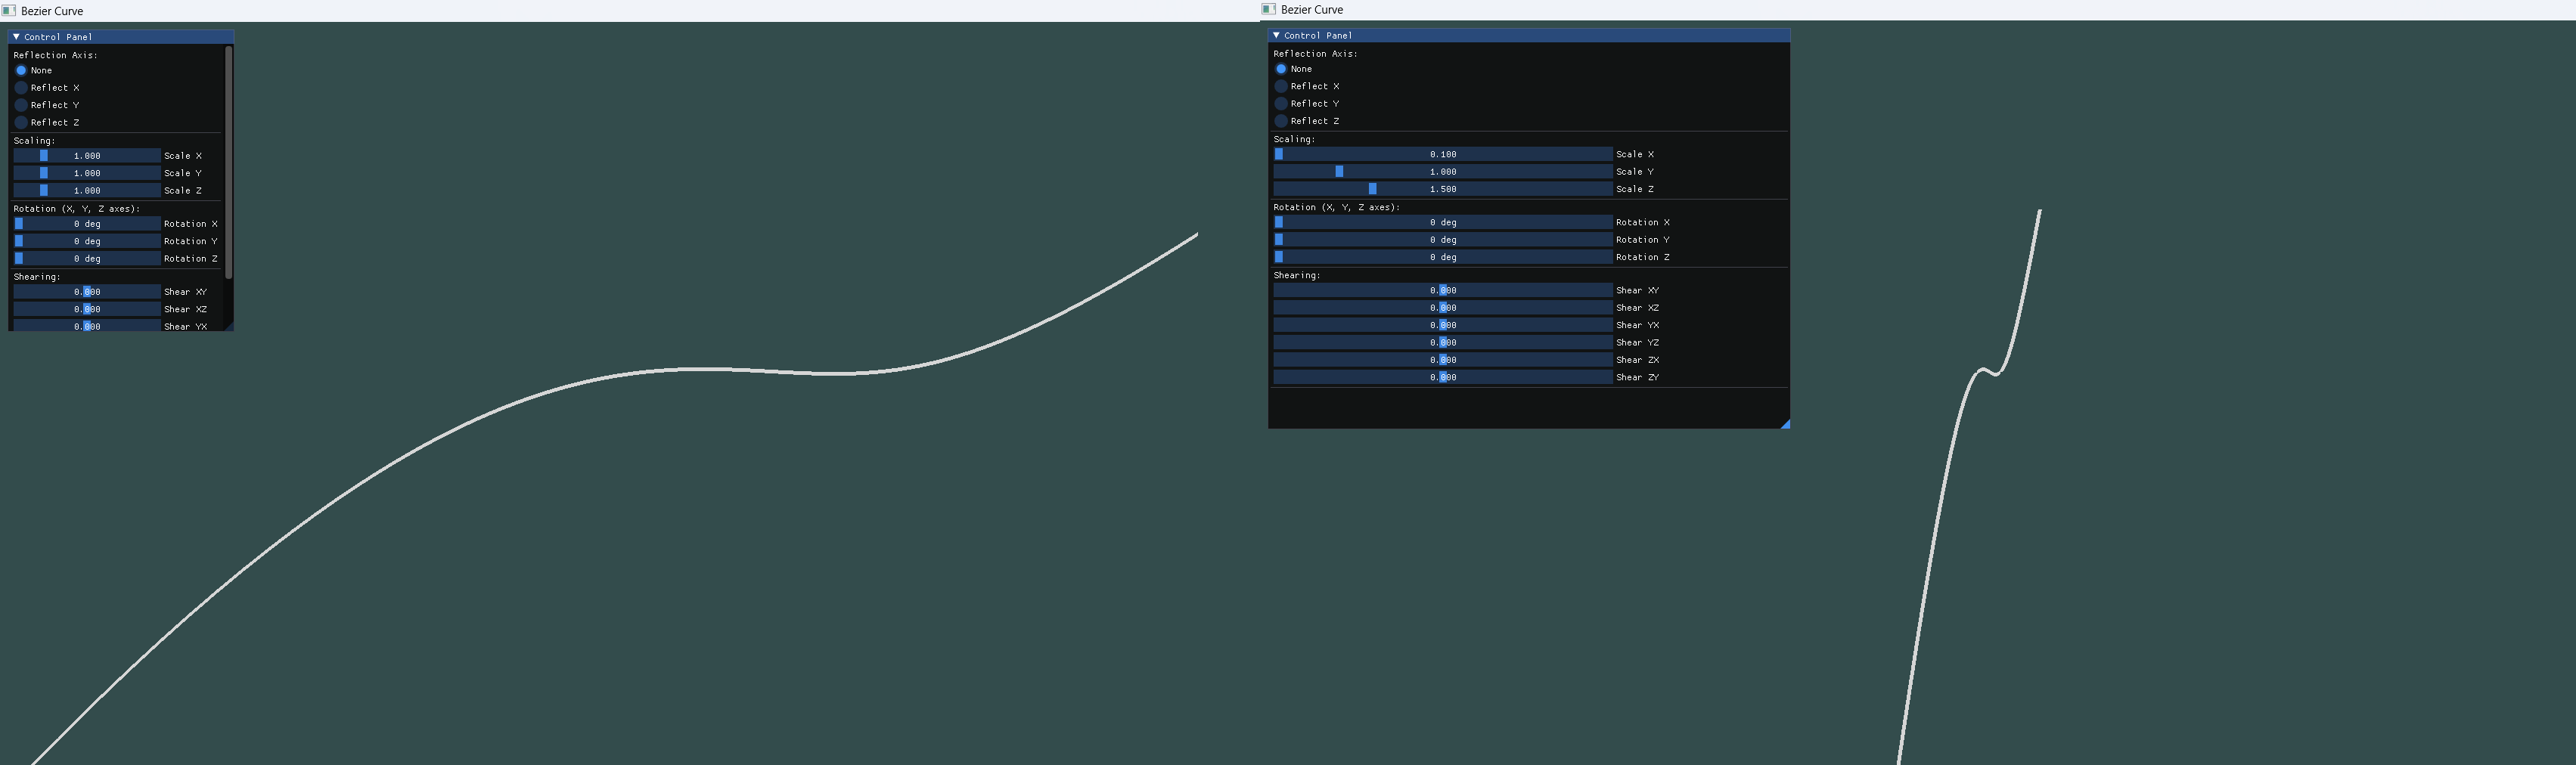
\includegraphics[width=1\linewidth]{tc1.png}
    \caption{Graph of $\mathbf{B}$ (left) and $\mathbf{B}$ scaled with the factor $k_x = 0.1$, $k_y = 1$, $k_z = 1.5$ (right).}
\end{figure}
\begin{figure}[htb!]
    \centering
    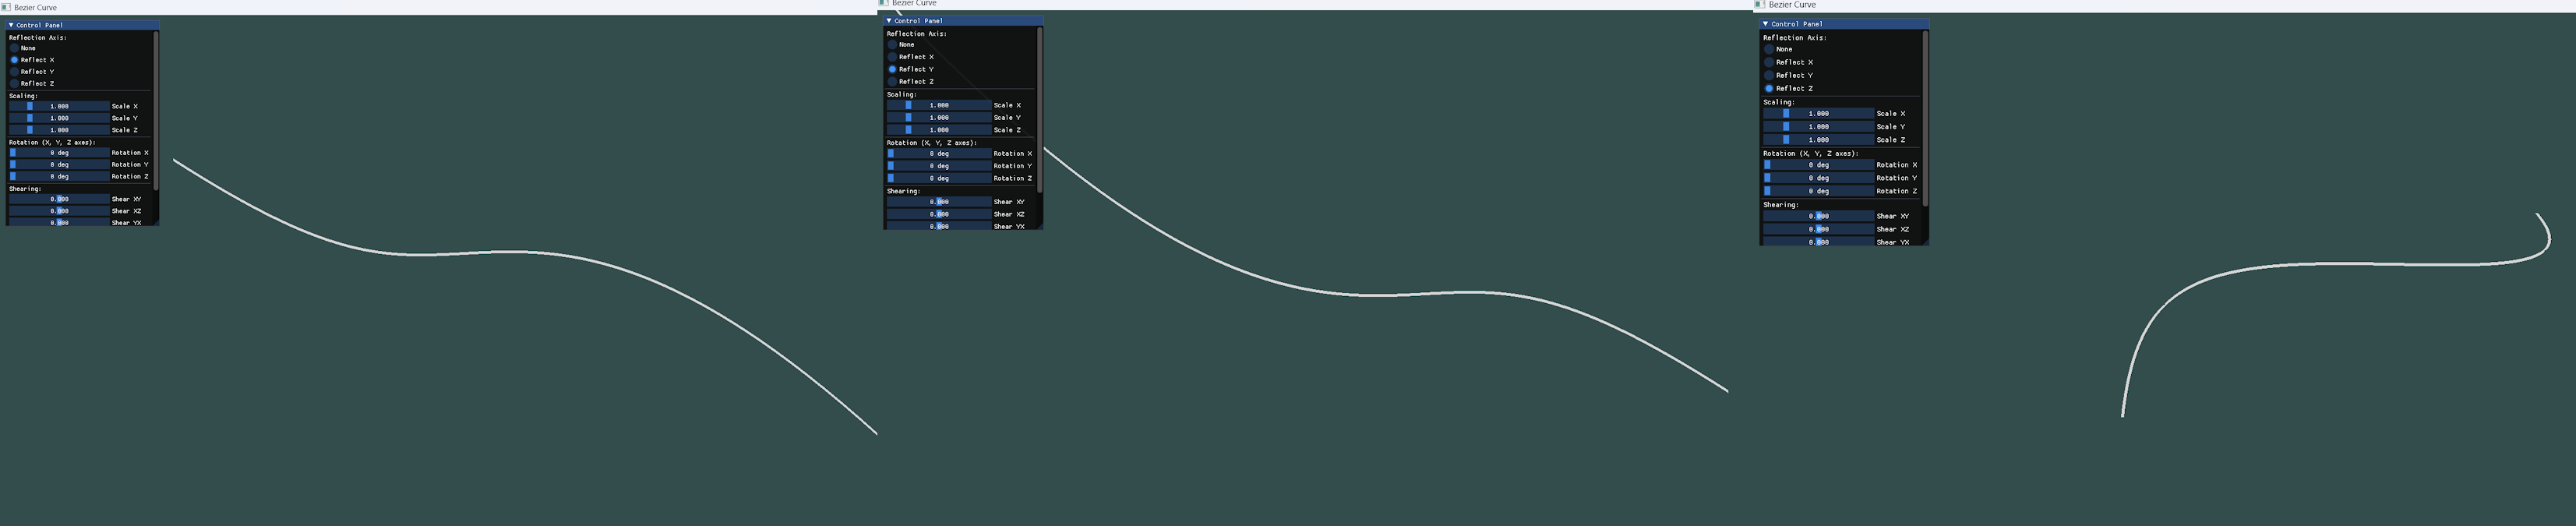
\includegraphics[width=1\linewidth]{tc2.png}
    \caption{$\mathbf{B}$ reflected to the $x$, $y$, and $z$ axes, from left.}
\end{figure}
\begin{figure}[htb!]
    \centering
    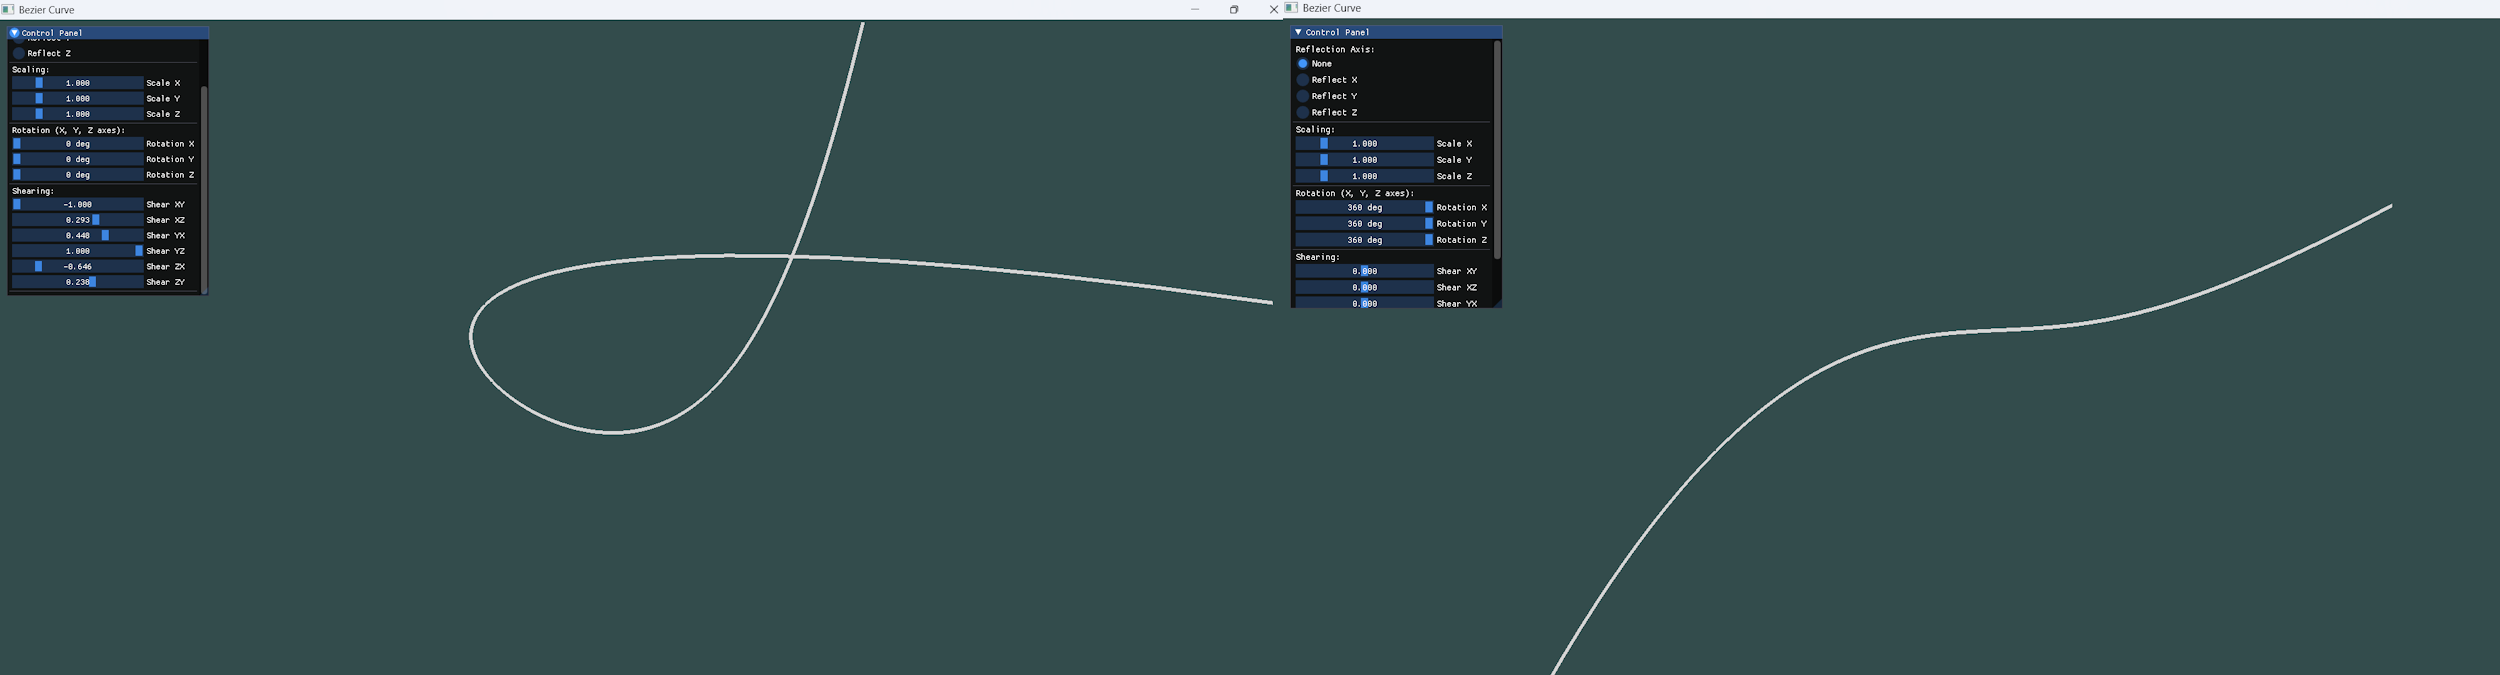
\includegraphics[width=1\linewidth]{tc3.png}
    \caption{Demonstration of shear mapping (left) and rotation (right).}
\end{figure}
\section{Conclusion}
This paper presents a simple yet powerful way to create and manipulate Bézier curves in three dimensions with the help of vector mathematics and linear transformations. Considering the affine properties of Bézier curves, we made an indication of how to perform linear transformations onto the whole curve smoothly passing the transformations of its control points. At the same time, the use of quaternions for rotation goes the extra mile, giving an immediate solution to typical problems, including gimbal lock, with better computational performance than conventional matrices and Euler angles.

Implemented through a Python-based OpenGL GUI using GLFW and ImGUI, our work established an interactive environment for the real-time visualization and manipulation of cubic Bézier curves. This was achieved with the controls on a graphical interface through which transformation parameters could be varied along the x, y, and z axes, thus making geometric transformations easily accessible in 3D space.

The demonstration further strengthen the theoretical foundation for the practical use of vector-based representations in concert with techniques from linear algebra and quaternion algebra for computer graphic applications. Just as it lays a hardcore background for the manipulation of Bézier curves, so too will it offer support for still higher modeling and animation work relating to three dimensions in 3D domains.

    
\section{Appendix}
    The GitHub repository containing the source code for a simple demonstration, as well as the source of several images in this paper, can be accessed \href{https://github.com/nayakazna}{\color{blue} here}. The repository also includes detailed instructions on how to run the code.

\section{Acknowledgment}

\begin{quote}
    \textit{Untaian benang takdir mempersatukan kita, \\
    Teknik Informatika berjiwa kesatria.}
\end{quote}

I would like to express my heartfelt gratitude to Dr. Ir. Rinaldi Munir, M.T., the lecturer of my IF2123 Aljabar 
Linear dan Geometri (Linear and Geometry Algebra) class, for his guidance throughout my first semester 
in the Informatics Engineering program at ITB. Moreover, I present my warmest gratitude to Ayesach Svarosstinez
Adhyatman for inspiring the creation of this paper and for her continuous encouragement and support throughout 
its development. Lastly, thanks to Beyoncé.

% Please number citations consecutively within brackets \cite{b1}. The 
% sentence punctuation follows the bracket \cite{b2}. Refer simply to the reference 
% number, as in \cite{b3}---do not use ``Ref. \cite{b3}'' or ``reference \cite{b3}'' except at 
% the beginning of a sentence: ``Reference \cite{b3} was the first $\ldots$''

% Number footnotes separately in superscripts. Place the actual footnote at 
% the bottom of the column in which it was cited. Do not put footnotes in the 
% abstract or reference list. Use letters for table footnotes.

% Unless there are six authors or more give all authors' names; do not use 
% ``et al.''. Papers that have not been published, even if they have been 
% submitted for publication, should be cited as ``unpublished'' \cite{b4}. Papers 
% that have been accepted for publication should be cited as ``in press'' \cite{b5}. 
% Capitalize only the first word in a paper title, except for proper nouns and 
% element symbols.

% For papers published in translation journals, please give the English 
% citation first, followed by the original foreign-language citation \cite{b6}.

\begin{thebibliography}{00}
\bibitem{hughes} J.F. Hughes, \textit{Computer Graphics: Principles and Practice}, 3\textsuperscript{rd} ed. Reading, MA: Addison-Wesley, 1995, pp. 1--10, 598.
\bibitem{eck} D.J. Eck, \textit{Introduction to Computer Graphics}, v.1.4. Available: \href{https://math.hws.edu/eck/cs424/downloads/graphicsbook-linked.pdf}{https://math.hws.edu/eck/cs424/downloads/graphicsbook-linked.pdf}. [Accessed: Dec. 27, 2024 23:30].
\bibitem{hci} A. Sears and J. A. Jacko, \textit{The Human–Computer Interaction Handbook: Fundamentals, Evolving Technologies and Emerging Applications}, 2nd ed. Boca Raton, FL, USA: CRC Press, 2007, p. 5. Available (preview): \href{https://books.google.co.id/books?id=A8TPF_O385AC&pg=PA1&hl=id&source=gbs_toc_r&cad=2#v=onepage&q&f=false}{https://books.google.co.id/books?id=A8TPF\_O385AC}. [Accessed: Dec. 28, 2024 00:30].
\bibitem{acm}  K. A. Frenkel, "An interview with Ivan Sutherland," \textit{Commun. ACM}, vol. 32, pp. 712-714, 1989.
\bibitem{sutherland} I. E. Sutherland, "Sketchpad: A man-machine graphical communication system," in \textit{Proc. May 21-23, 1963, Spring Joint Computer Conference (AFIPS '63 Spring)}, New York, NY, USA, 1963, pp. 329–346. doi: \href{https://doi.org/10.1145/1461551.1461591}{10.1145/1461551.1461591}. [Accessed: Dec. 28, 2024 00:55].
\bibitem{history} K. Sathyanarayana and G. V. V. Ravi Kumar, "Evolution of Computer Graphics and Its impact on Engineering Product Development" in \textit{2008 Fifth International Conference on Computer Graphics, Imaging and Visualisation}, Penang, Malaysia, 2008, pp. 32-37, doi: \href{https://ieeexplore.ieee.org/stamp/stamp.jsp?tp=&arnumber=4626981}{10.1109/CGIV.2008.67}. [Accessed: Dec. 28, 2024 00:57].
\bibitem{siggraph} D. J. Kasik, M. C. Whitton and C. R. Johnson, "The Big 50: Celebrating 50 ACM SIGGRAPH Conferences" in \textit{IEEE Computer Graphics and Applications}, vol. 43, no. 04, pp. 12-80, July-Aug. 2023, doi: \href{https://doi.ieeecomputersociety.org/10.1109/MCG.2023.3266086}{10.1109/MCG.2023.3266086}. [Accessed: Dec. 28, 2024 01:10].
\bibitem{cgi-movie} Z. Sun, “What Does CGI Digital Technology Bring to the Sustainable Development of Animated Films?” in \textit{Sustainability}, vol. 15, no. 14. MDPI AG, p. 10895, Jul. 11, 2023. doi: \href{https://www.mdpi.com/2071-1050/15/14/10895}{10.3390/su151410895}. [Accessed: Dec. 28, 2024 01:13].
\bibitem{bezier} Å. Kilicoglu, S. Åženyurt (2020). On the involute of the cubic Bezier curve by using matrix representation in E3. \textit{European Journal of Pure and Applied Mathematics}, 13(2), 216–226. doi: \href{https://doi.org/10.29020/nybg.ejpam.v13i2.3648}{10.29020/nybg.ejpam.v13i2.3648}. [Accessed: Dec. 30, 2024 03:26].
\bibitem{strang} G. Strang, \textit{Introduction to Linear Algebra}, 6\textsuperscript{th} ed. Wellesley, MA: Wellesley-Cambridge Press, 2023.
\bibitem{lengyel} E. Lengyel, \textit{Mathematics for 3D Game Programming and Computer Graphics}, 3\textsuperscript{rd} ed. Boston, MA, USA: Cengage Learning, 2011, pp. 317--329. ISBN: 978-1-4354-5886-4.
\bibitem{quat} [1] R. Goldman, “Understanding quaternions,” \textit{Graphical Models}, vol. 73, no. 2. Elsevier BV, pp. 21–49, Mar. 2011. doi: \href{https://www.researchgate.net/publication/220632454_Understanding_quaternions}{10.1016/j.gmod.2010.10.004}.
\bibitem{affine1} R. T. Rockafellar, \textit{Convex analysis}. Princeton, NJ: Princeton University Press, 1970. Available: \href{https://archive.org/details/convexanalysis0000rock}{https://archive.org/details/convexanalysis0000rock}. [Accessed Jan. 2 2025 04:11].
\bibitem{affine2} Reinhard Schultz, \textit{Affine transformations and convexity}, n.d. Available: \href{https://math.ucr.edu/~res/math145A-2014/affine+convex.pdf}{https://math.ucr.edu/\~res/math145A-2014/affine+convex.pdf}. [Accessed: Jan. 2, 2025 03:38].
\bibitem{affine2} D. Bertsekas, A. Nedic, and A. Ozdaglar, Convex analysis and optimization. Belmont, MA: Athena Scientific, 2003.
\bibitem{rot} S. Kim and M. Kim, “Rotation Representations and Their Conversions,” IEEE Access, vol. 11, pp. 6682–6699, 2023. doi: \href{https://ieeexplore.ieee.org/document/10019271}{10.1109/ACCESS.2023.3237864
}. [Accessed: Dec. 28, 2024 05:02].
\bibitem{galier} J. Galier, \textit{Curves and Surfaces In Geometric Modeling: Theory And Algorithms}, 2\textsuperscript{nd} ed. Accessed Dec. 28 2024. [Online]. Available: \href{https://www.cis.upenn.edu/~jean/geomcs-v2.pdf}{https://www.cis.upenn.edu/~jean/geomcs-v2.pdf}. [Accessed: Dec. 25, 2024 18:22].
\end{thebibliography}

% \newpage

\section*{Declaration of Originality}
I hereby declare that the work presented in this paper is entirely my own. It is not a copy, translation, or adaptation of any other author's work, and it does not constitute plagiarism.

\begin{flushright}
    Bandung, December, 28\textsuperscript{th} 2024 \\  
    Z. Nayaka Athadiansyah – 13523094
\end{flushright}

\end{document}
